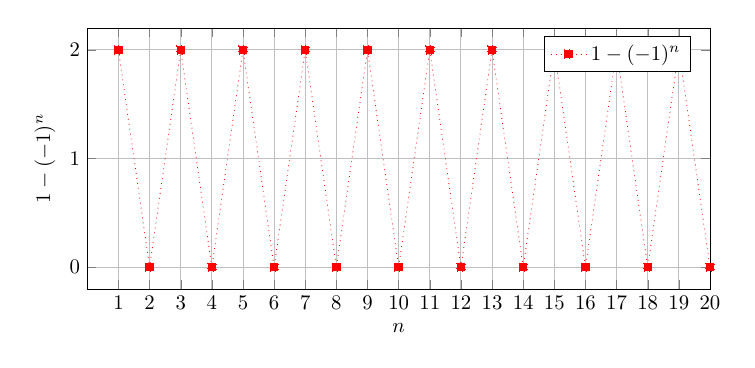
\begin{tikzpicture}[scale=.75]
	\begin{axis}[
		xlabel={$n$},
		ylabel={$1-(-1)^n$},
		ymin=-.2, ymax=2.2,
		xmin=0, xmax=20,
		xtick={1,2,...,20},
		ytick={0,1,2},
		grid=major,
		width=\textwidth,
		height=6cm,
		domain=1:20,
		samples=20,
		legend pos=north east,
		]
		\addplot[red, mark=square*, dotted, mark options={fill=red}] {1 - (-1)^x};
		\addlegendentry{$1-(-1)^n$};
		
		% Draw horizontal line showing upper bound (y=1)
		%		\addplot[dashed, magenta, line width=.5mm] coordinates {(0,1) (30,1)};
		%		\node[magenta] at (axis cs: 3,1.1) {Upper Bound $1$};
		
		% Draw horizontal line showing lower bound (y=0)
		%		\addplot[dashed, cyan, line width=.5mm] coordinates {(0,0) (30,0)};
		%		\node[cyan] at (axis cs: 3,-0.1) {Lower Bound $0$};	
	\end{axis}
\end{tikzpicture}